\documentclass{article}
\usepackage{tikz}

\title{Segment Trees in Algorithmic Problems}
\author{Piotr Szczepaniak}
\date{\today}

\begin{document}

\maketitle

\tableofcontents

\begin{abstract}
This document provides an overview of segment trees. In the first place
I will describe some algebraic topics which are necessary for better
understanding how and why segment trees works. This knowledge will be useful
for reading the rest of the paper where We will dive into different kinds of trees.
For each structure, I will explain how it work and how to apply it to problems.
Then, I will look at each structure's time complexity and space complexity.
\end{abstract}

\section{Foundations of Segment Trees}
A segment tree is a binary tree used for storing information about segments. 
To efficently retrieve or update informations about elements stored 
in segment tree we can perform various operations, the 
most common of which is the range query, range update or point update
(which is sipler case of range update). One of the examples of use can be maximum value of 
elements in given range or sum of elements in given range.


\begin{center}
    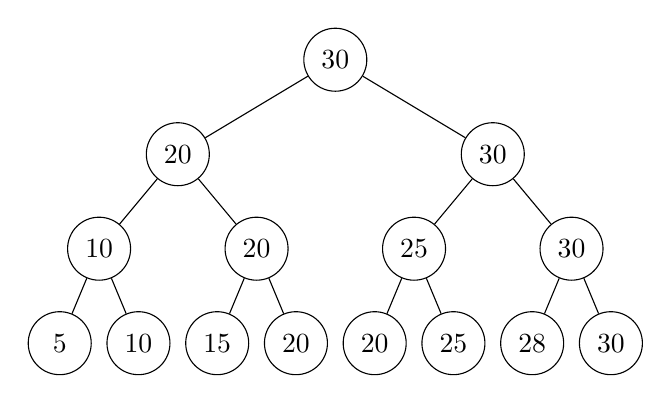
\begin{tikzpicture}[
      level distance=1.2cm,
      level 1/.style={sibling distance=4cm},
      level 2/.style={sibling distance=2cm},
      level 3/.style={sibling distance=1cm},
      every node/.style={draw,circle,minimum size=8mm,inner sep=1pt}
    ]
    
    % Root node with max value
    \node {30}
        child {node {20}
            child {node {10}
                child {node {5}}
                child {node {10}}
            }
            child {node {20}
                child {node {15}}
                child {node {20}}
            }
        }
        child {node {30}
            child {node {25}
                child {node {20}}
                child {node {25}}
            }
            child {node {30}
                child {node {28}}
                child {node {30}}
            }
        };
    
    \end{tikzpicture}
\end{center}

\subsection{Operation types}


\subsection{Monoids}
A monoid \( (S, e, \ast) \) is a set equipped with an associative binary operation \( S \times S \to S \) and
an identity element \(e\). 
\begin{itemize}
    \item \textbf{Associativity} \\
    For all \( a, b, c \in S \), \( (a \ast b) \ast c = a \ast (b \ast c) \).
    \item \textbf{Identity element} \\
    There exists an element \( e \in S \) such that for all \( a \in S \), \( a \ast e = e \ast a = a \).
\end{itemize}


\end{document}